%%%%%%%%%%%%%%%%%%%%%%%%%%%%%%%%%%%%%%%%%%%%%%%%%%%%%%%%%%%%%%%%%%%%%%%%%%%%%%%%
%2345678901234567890123456789012345678901234567890123456789012345678901234567890
%        1         2         3         4         5         6         7         8

\documentclass[letterpaper, 10 pt, conference]{ieeeconf}  % Comment this line out
                                                          % if you need a4paper
%\documentclass[a4paper, 10pt, conference]{ieeeconf}      % Use this line for a4
                                                          % paper

\IEEEoverridecommandlockouts                              % This command is only
                                                          % needed if you want to
                                                          % use the \thanks command
\overrideIEEEmargins
% See the \addtolength command later in the file to balance the column lengths
% on the last page of the document



% The following packages can be found on http:\\www.ctan.org
%\usepackage{graphics} % for pdf, bitmapped graphics files
%\usepackage{epsfig} % for postscript graphics files
%\usepackage{mathptmx} % assumes new font selection scheme installed
%\usepackage{times} % assumes new font selection scheme installed
%\usepackage{amsmath} % assumes amsmath package installed
%\usepackage{amssymb}  % assumes amsmath package installed
\usepackage{graphicx}
\usepackage{listings}
\usepackage{caption}
\usepackage{hyperref}

\title{\LARGE \bf
Condorcet Fusion: an implementation
}

%\author{ \parbox{3 in}{\centering Huibert Kwakernaak*
%         \thanks{*Use the $\backslash$thanks command to put information here}\\
%         Faculty of Electrical Engineering, Mathematics and Computer Science\\
%         University of Twente\\
%         7500 AE Enschede, The Netherlands\\
%         {\tt\small h.kwakernaak@autsubmit.com}}
%         \hspace*{ 0.5 in}
%         \parbox{3 in}{ \centering Pradeep Misra**
%         \thanks{**The footnote marks may be inserted manually}\\
%        Department of Electrical Engineering \\
%         Wright State University\\
%         Dayton, OH 45435, USA\\
%         {\tt\small pmisra@cs.wright.edu}}
%}

\author{Marco Alfonso$^{1}$ (1151026), Davide Martini$^{1}$ (1151502) and Giovanni Mazzocchin$^{2}$ (1156318)% <-this % stops a space
\thanks{$^{1}$Department of Information Engineering, University of Padua
        }%
\thanks{$^{2}$Department of Mathematics, University of Padua}
}%


\begin{document}



\maketitle
\thispagestyle{empty}
\pagestyle{empty}


%%%%%%%%%%%%%%%%%%%%%%%%%%%%%%%%%%%%%%%%%%%%%%%%%%%%%%%%%%%%%%%%%%%%%%%%%%%%%%%%
\begin{abstract}

The goal of this work is to implement, compare and evaluate different score-based fusion strategies with an advanced rank-based technique described by Montague and Aslam \cite{c1}: the "Condorcet procedure".
Our results show that this advanced strategy
performs similarly to basic fusion methods in most scenarios on TIPSTER collection.
Thus, we claim that plain methods such as CombSUM and CombMNZ still provide a better trade-off between quality of the outcomes and ease of implementation.

\end{abstract}


%%%%%%%%%%%%%%%%%%%%%%%%%%%%%%%%%%%%%%%%%%%%%%%%%%%%%%%%%%%%%%%%%%%%%%%%%%%%%%%%
\section{INTRODUCTION}
The ranking fusion problem is encountered in many situations and a prominent one is \textit{metasearch}. It aims to combine the retrieval results returned by different IRS (Information Retrieval Systems) in order to produce a fused ranked list of documents whose effectiveness measures are improved. 

This problem implies several issues like the normalization of relevance scores assigned by input IRS, the choice of a fusion strategy and the evaluation of the output result in order to select the best technique for the application task.

Several normalization and ranking fusion methods have been proposed in literature. In this paper we describe basic score normalization techniques proposed by Lee \cite{c3}. Moreover, we introduce basic fusion strategies which rely on similarity values like CombMAX, CombMIN, CombMED, CombSUM, CombANZ and CombMNZ. Finally we present the Condorcet fusion advanced technique described by Montague and Aslam \cite{c1}, which exploits documents' ranks.

The goal of this work is to implement the previously mentioned fusion strategies in order to compare them evaluating their output through usual metrics.


\section{Score normalization}
In rank fusion, we consider different IRS whose output results are combined into a new ranked list of documents. Since input systems may use different IR models, the relevance scores given to the same document for a specific topic could be incomparable.
For example, they may be on different scales, in different ranges of values or distributed differently. 
In order to satisfy this issue, relevance score normalization is applied to make them comparable across input systems. 

Montague and Aslam \cite{c4} proposed several normalization techniques, however, we implemented the normalization methods described by Lee \cite{c3} to each retrieval result. At first, the author proposed to normalize each similarity score by the maximum similarity value in a retrieval result.
$$
{Max\_Norm = {Old\_Sim \over Maximum\_Sim}}
$$ 
The former strategy coincides only the upper bounds, thus the author presents a more reasonable approach which coincides also lower bounds.
$$
{Min\_Max\_Norm = {{Old\_Sim - Minimum\_Sim} \over {Maximum\_Sim - Minimum\_Sim}}}
$$
All the results presented in this work are obtained using $Min\_Max\_Norm$ technique, whose application was the first step after the creation and the parsing of each input run. 

\section{Basic score-based fusion strategies}

In our work, we implemented six fusion techniques that rely on documents' similarity values in order to build the combined retrieval result. These strategies which were presented in \cite{c2}, are briefly described in this section and summarized in the following table.

\begin{table}[h]
\caption{Score-based fusion strategies}
\label{table_example}
\begin{center}
\begin{tabular}{|c|c|}
\hline
Strategy & Definition\\
\hline
CombMAX &  max (Similarity Values)\\
\hline
CombMIN & min (Similarity Values)\\
\hline
CombSUM & sum (Similarity Values)\\
\hline
CombMED & median (Similarity Values)\\
\hline
CombANZ & CombSUM / number of non-zero similarity values\\
\hline
CombMNZ & CombSUM * number of non-zero similarity values\\
\hline
\end{tabular}
\end{center}
\end{table}


In order to explain the idea behind these methods, let $d$ be a document retrieved for a specific topic $t$ by at least one of the $k$ input systems that must be combined. These strategies assign to $d$ a new score considering the normalized ones obtained from all $k$ runs. 

CombMIN looks for the minimum similarity value of $d$, while CombMAX focuses on the maximum score. CombMIN aims to minimize the effect that a non-relevant document would be highly ranked, while CombMAX goal is the opposite. 
The CombMED method tries to handle both the issues pointed out by CombMIN and CombMAX considering the median similarity score of document $d$ over $k$ runs.
The most important aspect of CombMED is that it does not select one of the $k$ scores, but it assigns to $d$ a score which depends on all the $k$ similarity values.
CombSUM is very similar to CombMED since it considers the summation over all similarity scores assigned to $d$. Moreover, CombANZ computes the average of the non-zero scores given to $d$: this method ignores the effects of single runs among the $k$s that fail to retrieve $d$.
Finally, CombMNZ assigns to $d$ the product of CombSUM's score and the number of non-zero similarities given to $d$: in this way, this strategy provides higher weights to documents retrieved by multiple IRS. 

\section{Condorcet}

The work by Aslam and Montague \cite{c1} applies some ideas stemming from \textit{Social Choice Theory} (whose origins date back to $18^{th}$ century's Condorcet's and Borda's investigations) to the \textit{metasearch} framework.

In particular, their work focuses on the so called "Condorcet voting algorithm", a majoritarian method used as a metaphor for two algorithms suggested by these authors.
Firstly, they devise a "Simple Majority Runoff" algorithm serving as a comparator between a given couple of documents (Listing 1). Actually, this procedure accepts two documents ($d_1$ and $d_2$) and runs a loop of comparisons among the ranks yielded by $k$ various search systems, thus bestowing win on the document which ranks above the other one more frequently.

\lstset{
language=C++,
basicstyle=\small\ttfamily,
numbers=left,
numbersep=5pt,
xleftmargin=20pt,
frame=tb,
framexleftmargin=20pt
}

\renewcommand*\thelstnumber{\arabic{lstnumber}:}

\captionsetup[lstlisting]{labelfont=bf,singlelinecheck=off,labelsep=space}

\begin{lstlisting}[caption={Simple Majority Runoff}]
count = 0
for each of the k search systems do
    if(k ranks d1 above d2) count++
    if(k ranks d2 above d1) count--
if(count > 0) rank d1 better than d2
else rank d2 better than d1
\end{lstlisting}


After defining this first building block, the paper in question proposes two \textit{metasearch} algorithms. The former method (deemed as \textit{theoretic} by the authors) starts by creating a \textit{semi-complete} graph, dubbed \textit{Condorcet graph}, whose number of nodes is equal to the number of documents. \newline Its edges are organized as follows: for each pair of documents $(d_1, d_2)$, an edge exists from node $d_1$ to $d_2$ if $d_1$ ranks above (receives at least as many votes as) $d_2$ most often. In order to compute the final documents ranking, at least a Hamiltonian path through the Condorcet graph should be found.

\begin{lstlisting}[caption={Theoretic Condorcet Metasearch}]
for all pairs (d1, d2) of documents do
    Use Listing 1 to compute the graph
Compute Hamiltonian path of the graph
\end{lstlisting}

Considering a \textit{metasearch} problem with $k$ IRS (voters) on a collection of $n$ documents (candidates), it can be shown that only the \textit{Condorcet graph} creation has a $O(n^{2}k)$ time complexity. It's clear that its implementation is impractical for big collections, thus the authors designed the \textit{Condorcet-fuse} algorithm, which runs in $O(nkln(n))$. The key idea is to sort the nodes using the "Simple Majority Runoff" algorithm as comparison function without generating the entire \textit{Condorcet graph}. In this work we implemented the \textit{Condorcet-fuse} strategy using a simple \textit{MergeSort} algorithm, even if Aslam and Montague used \textit{QuickSort} to prove its correctness. 

\begin{lstlisting}[caption={Condorcet-fuse}]
Create a list L of all the documents
Sort(L) with Listing 1 as comparator
Output the sorted list of documents
\end{lstlisting}

\section{Implementation issues}
This work is based on disk 4 and 5 of TIPSTER collection (without Congressional Record) and considering TREC7 topics from 351 to 400. In order to pursuit our goal, we faced and solved some issues that we briefly describe in this section. All the implementation details and the related source code are available at \textit{https://github.com/KondorPhase/KondorFusion}.

\subsection{Input runs generation}
At first, in order to create ten different input IRS, we generated ten different runs that represent their retrieval results using \textit{Terrier}, a popular open source search engine. These runs differ in the model and in the indexing procedure used by \textit{Terrier} to create them. A list with our choices on IR models follows:
\begin{itemize}
\item \textbf{BM25}: the BM25 probabilistic model;
\item \textbf{Hiemstra\_LM}: Hiemstra's language model;
\item \textbf{LGD (DFR)}: a log-logistic DFR model;
\item \textbf{TF\_IDF}: the $tf\times idf$ weighting function;
\item \textbf{InL2 (DFR)}: inverse document frequency model for randomness.
\end{itemize}

Furthermore, we generated two runs per model that differ in some indexing steps. We were interested in observing the behavior of the fusion strategies when \textit{stemming} or \textit{stopwords removal} were applied. Thus, we instructed \textit{Terrier} to create two runs for each selected model: one as result of a system that uses \textit{stemming} without \textit{stopwords removal} and vice versa.

\subsection{Parser Structure}
\begin{figure}[!htbp]
\centering
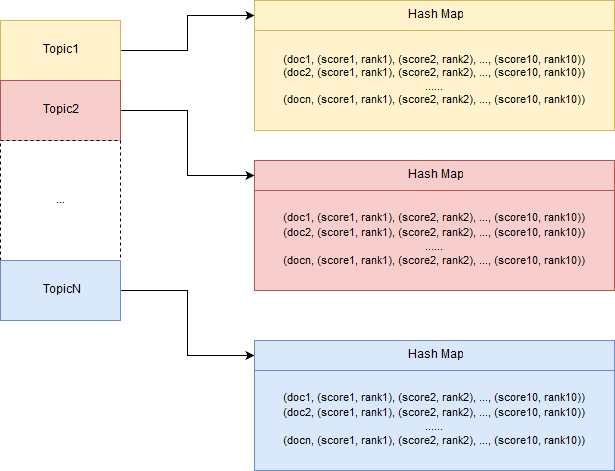
\includegraphics[width=0.5\textwidth]{structure}
\caption{Parser Data Structure}
\label{FIG:Data Structure}
\end{figure}

In order to perform the different fusion strategies, we had to write a parser which is able to read and store all the useful information provided by initial runs. Thus, we designed the data structure depicted in Figure 1 which is composed by:
\begin{itemize}
\item an array that contains an ordered list of all topics with a reference that points to an hash map; 
\item an hash map for each topic that has \textit{document id} as key and a list of \textit{(score, rank)} couples: one for each of the ten input runs.
\end{itemize}


Furthermore, we performed the \textit{Min\_Max\_Norm} normalization technique during the parsing phase: in this way the data structure stores the normalized documents' scores. This particular design choice eased the implementation of the fusion strategies. 

\subsection{Fusion strategies implementation}
As we have seen in the previous paragraphs, we had to implement six different score-based fusion techniques (Table 1) and then the  Condorcet fusion strategy. Thanks to the information stored in the parser data structure (Figure 1), the score-based fusion strategies are simple to realize since it is enough to follow their definition proposed in Table 1.

As we have seen in the IV section, there are two different algorithms that perform the Condorcet strategy. We chose to realize the Condorcet-fuse algorithm (Listing 3) since it provides a better time efficiency ($O(nkln(n))$). Its implementation is composed by three steps:
\begin{itemize}
\item the creation of a list of all documents which is already available using the parser data structure;
\item the creation of the comparator "Simple Majority Runoff" (Listing 1);
\item the sorting of documents using the comparator and \textit{MergeSort} algorithm.
\end{itemize}

Particular attention is dedicated to implement the "Simple Majority Runoff" comparator because not all runs retrieve the same documents for a given topic. In order to explain this scenario, consider a topic $t$ and two documents $d_1$ (retrieved by the system $i$) and $d_2$ (not retrieved by the system $i$). In this example, $d_1$ is ranked by $i$ ($rank1$) while $d_2$ is not ($rank2 = null$), thus the comparisons performed by "Simple Majority Runoff" algorithm can not be computed. Our solution to this critical issue is to consider $d_1$ ranked above $d_2$ since it has been retrieved while $d_2$ has not. Listing 4 briefly describes our solution which considers also the vice versa. A particular situation may happen in case both $d_1$ and $d_2$ are not retrieved by the system $i$ (they appear in the parser structure since they are retrieved by other systems). Our solution makes the variable $count$ remain unchanged because we can not say what document has a better rank. 

\begin{lstlisting}[caption={Simple Majority Runoff implementation detail}]
if(rank1 == null || rank2 == null){
    if(rank2 == null)
        count++;
    if(rank1 == null)
        count--;
}
else {
    if(rank1 < rank2)
        count++;
    else if(rank1 > rank2)
        count--;
}
\end{lstlisting}

\section{Evaluation and results analysis}
The results described in this section are obtained thanks to the \textit{trec\_eval} tool, which computes many effectiveness measures.

In order to provide a more descriptive comparison between all the presented fusion strategies, we evaluated and divided the fused runs by their origin: 
\begin{itemize}
\item generated by five runs with only the \textit{stemming} indexing phase;
\item generated by five runs with only the \textit{stopwords removal} indexing phase;
\item generated by all ten runs.  
\end{itemize}

\begin{figure}[!htbp]
\centering
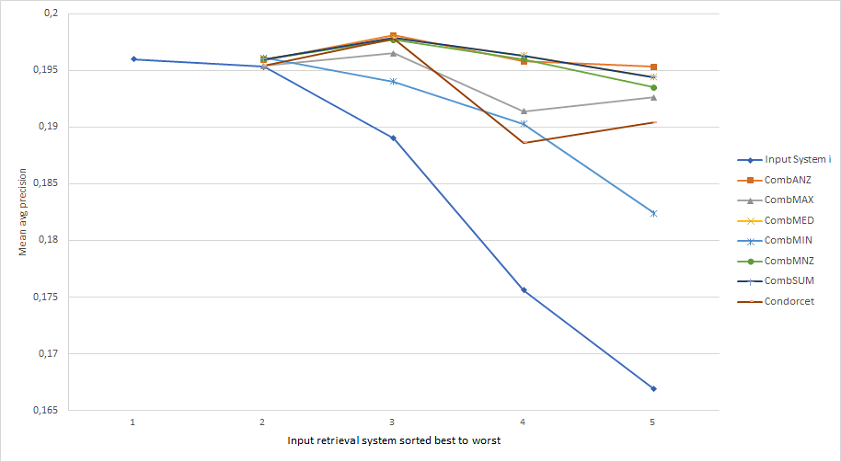
\includegraphics[width=0.5\textwidth]{stemmerMap}
\caption{MAP plot fusing five runs with \textit{stemming} in order}
\label{FIG:Combining five runs with stemming in order}
\end{figure}

\begin{figure}[!htbp]
\centering
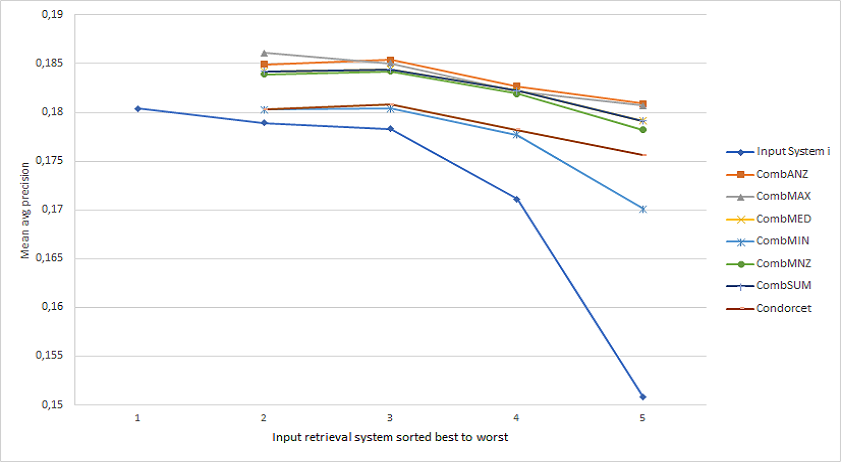
\includegraphics[width=0.5\textwidth]{stopwordMap}
\caption{MAP plot fusing five runs with \textit{stopwords removal} in order}
\label{FIG:Combining five runs with stopwords removal in order}
\end{figure}

\begin{figure}[!htbp]
\centering
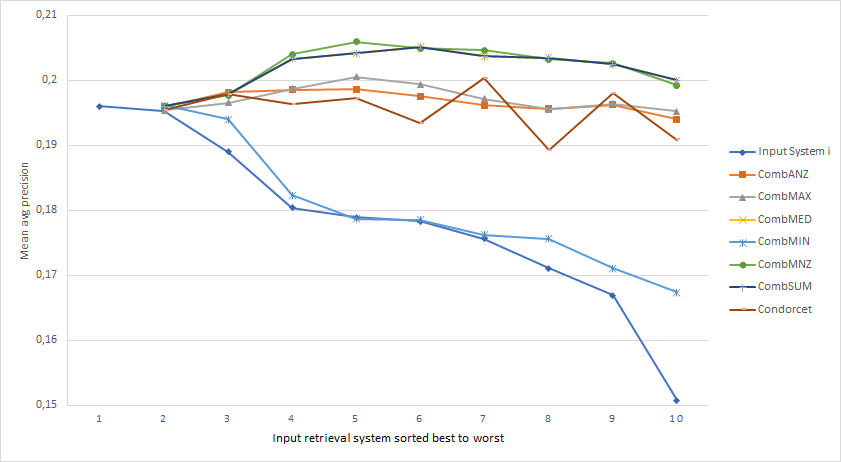
\includegraphics[width=0.5\textwidth]{run}
\caption{MAP plot fusing ten runs in order}
\label{FIG:Combining ten runs in order}
\end{figure}

\begin{figure}[!htbp]
\centering
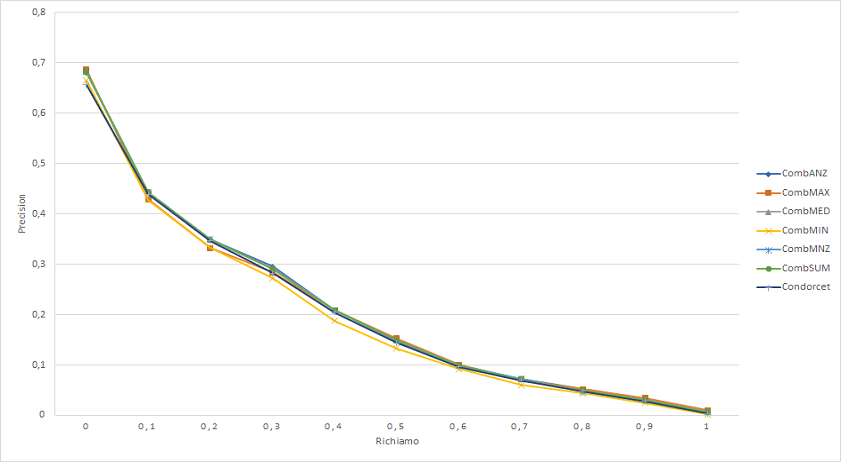
\includegraphics[width=0.5\textwidth]{RP5stemmer}
\caption{Interpolated RP curve fusing five runs with \textit{stemming}}
\label{FIG:Combining five runs with stemming in order}
\end{figure}

\begin{figure}[!htbp]
\centering
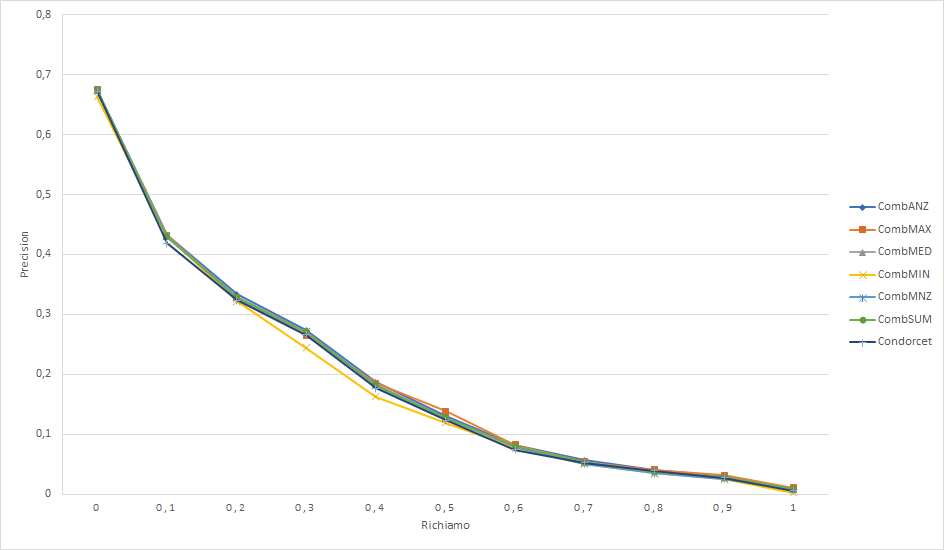
\includegraphics[width=0.5\textwidth]{RP5stopword}
\caption{Interpolated RP curve fusing five runs with \textit{stopwords removal}}
\label{FIG:Combining five runs with stopwords removal in order}
\end{figure}

\begin{figure}[!htbp]
\centering
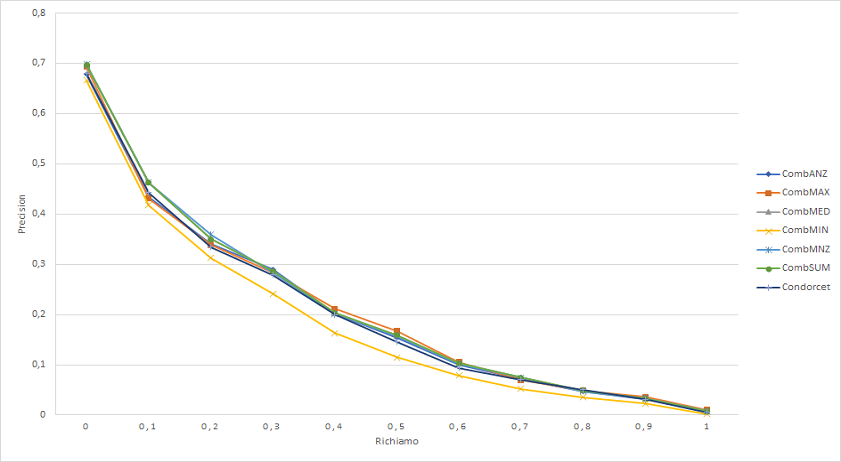
\includegraphics[width=0.5\textwidth]{RP10}
\caption{Interpolated RP curve fusing ten runs}
\label{FIG:Combining ten runs in order}
\end{figure}

\begin{figure}[!htbp]
\centering
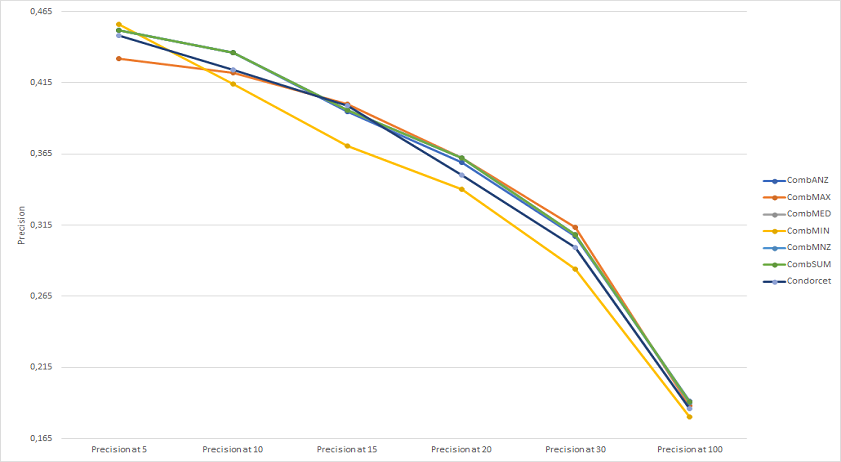
\includegraphics[width=0.5\textwidth]{precisionStemmer}
\caption{Precision at cutoff fusing five runs with \textit{stemming}}
\label{FIG:Combining five runs with stemming in order}
\end{figure}

\begin{figure}[!htbp]
\centering
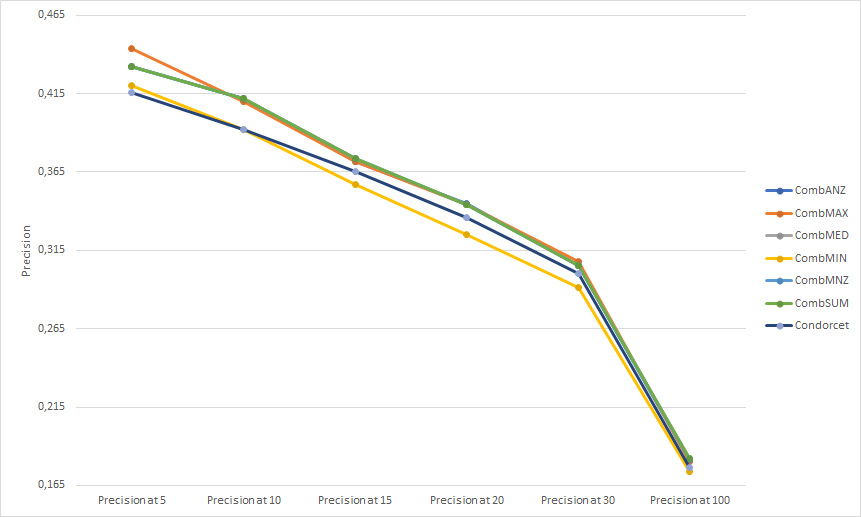
\includegraphics[width=0.5\textwidth]{precisionStopword}
\caption{Precision at cutoff fusing five runs with \textit{stopwords removal}}
\label{FIG:Combining five runs with stopwords removal in order}
\end{figure}

\begin{figure}[!htbp]
\centering
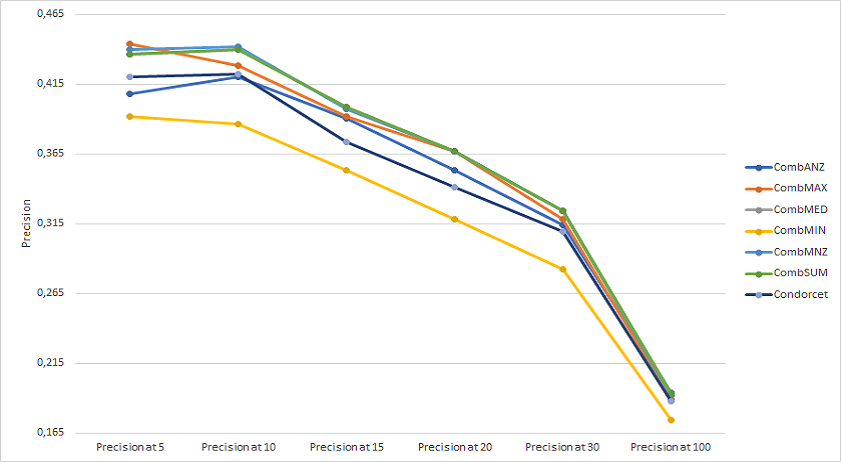
\includegraphics[width=0.5\textwidth]{precisionRun}
\caption{Precision at cutoff fusing ten runs}
\label{FIG:Combining ten runs in order}
\end{figure}

In this paper, we propose three types of graphical representation that consider all the information collected from our input runs and fused results:
\begin{itemize}
\item MAP plot obtained by fusing best-to-worst input runs (Figures 2, 3 and 4);
\item eleven point interpolated recall-precision curve (Figures 5, 6 and 7);
\item precision values at six different cutoffs (Figures 8, 9 and 10).
\end{itemize}



The graphs presented in figures 2, 3 and 4 should point out how the \textit{metasearch} algorithms perform when combining the input systems from the best to the worst in terms of MAP. In other words, they show the MAP obtained combining the top two systems, then the top
three, and so on. If we compare Figure 2 and 3, we can notice that both the score-based strategies and the Condorcet method perform better (in terms of absolute MAP value) when applied to systems that use \textit{stemming} instead of \textit{stopwords removal}. In Figure 2, the greatest MAP improvement in comparison with the best input system ($TF\_IDF$ model) is provided by CombANZ when fusing the top three input runs and it amounts to $1.07\%$. Moreover, we can state that CombMIN is the worst choice in this scenario even if it outperforms Condorcet strategy when combining the top four runs. As regards the fusion of input systems with \textit{stopwords removal} (Figure 3), CombMAX result improves by $3.16\%$ the MAP performance of the best input run ($LGD$ model) when it combines the top two systems. As for Figure 2, we claim that CombMIN provides the worst performances, but the other score-based strategies slightly outperform the Condorcet method. Finally, considering Figure 4, we can observe that fusion strategies like CombMNZ and CombSUM (which assumes the same MAP values as CombMED) provide the best performances with an improvement up to $4.54\%$ over the best input system ($TF\_IDF$ model with $stemming$), while CombMIN is definitely the worst one. Condorcet method performs similarly to CombMAX and CombANZ but presents interesting drops of the MAP values when new systems with \textit{stopwords removal} are added to the pool of the combined ones. 

The interpolated eleven point recall-precision curves shown in Figure 5 and 6 do not point out relevant differences between the fusion strategies. However, when considering all ten input runs (Figure 7), we can state that CombMIN is the worst fusion method especially considering its performances at recall $0.3$, $0.4$ and $0.5$.

Figure 8 shows that CombMAX result has the lowest precision value at cutoff $5$, but CombMIN is still the worst from cutoff $10$ up to $100$. The same can be said observing Figure 9, even if CombMIN performs similarly to Condorcet for cutoff $5$ and $10$. Finally combining all ten runs (Figure 10), we can notice that CombSUM, CombMED and CombMAX are the best fusion strategies, while CombMIN is confirmed to be the worst choice. Furthermore, Condorcet performs similarly to the other score-based strategies for high cutoff levels.

In conclusion we claim that strategies like CombMNZ and CombSUM provide a better trade-off between quality of the outcomes (respectively in terms of MAP and precision with cutoff) and ease of implementation than Condorcet fuse.



\addtolength{\textheight}{-12cm}   % This command serves to balance the column lengths
                                  % on the last page of the document manually. It shortens
                                  % the textheight of the last page by a suitable amount.
                                  % This command does not take effect until the next page
                                  % so it should come on the page before the last. Make
                                  % sure that you do not shorten the textheight too much.

%%%%%%%%%%%%%%%%%%%%%%%%%%%%%%%%%%%%%%%%%%%%%%%%%%%%%%%%%%%%%%%%%%%%%%%%%%%%%%%%



%%%%%%%%%%%%%%%%%%%%%%%%%%%%%%%%%%%%%%%%%%%%%%%%%%%%%%%%%%%%%%%%%%%%%%%%%%%%%%%%



%%%%%%%%%%%%%%%%%%%%%%%%%%%%%%%%%%%%%%%%%%%%%%%%%%%%%%%%%%%%%%%%%%%%%%%%%%%%%%%%

%%%%%%%%%%%%%%%%%%%%%%%%%%%%%%%%%%%%%%%%%%%%%%%%%%%%%%%%%%%%%%%%%%%%%%%%%%%%%%%%

\begin{thebibliography}{99}

\bibitem{c1} M. Montague, J. A. Aslam, Condorcet Fusion for Improved Retrieval. CIKM’02, November 4–9, 2002, McLean, Virginia, USA 
\bibitem{c2} E. A. Fox, M. P. Koushik, J. Shaw, R. Modlin, and
D. Rao. Combining evidence from multiple searches.
In D. Harman, editor, The First Text REtrieval
Conference (TREC-1), pages 319–328, Gaithersburg,
MD, USA, Mar. 1993. U.S. Government Printing
Office, Washington D.C.
\bibitem{c3} Lee, Joon Ho. Combining multiple evidence from different properties of weighting schemes. Proceedings
of the 18th annual international ACM SIGIR conference on Research and development in information retrieval. ACM, 1995.
\bibitem{c4} M. Montague, J. A. Aslam, Relevance Score Normalization for Metasearch. CIKM’OI, November 5-10,2001, Atlanta, Georgia, USA.
\end{thebibliography}




\end{document}
